\chapter{Industrial Management}

\textbf{Resorcess}
\begin{itemize}
    \item \url{https://hakan-kullven.webnode.se/}
    \item \url{https://www.youtube.com/watch?v=Q0o9S0q0Rr4}
    \item \url{https://www.youtube.com/watch?v=Kw-1nopchnA}
\end{itemize}

\newpage

\section{Verksamheter}
\textbf{Företags former}
\begin{figure}[H]
    \centering
    \includegraphics[width=12cm]{\imagesPath/företagsformer.png}
    \caption{Control without feedback. From \cite{im}}
\end{figure}


Note: om du med i ett handelsbolag eller kommanditbolag se till att du inte
har ett kompanions avtal med juridiskt ombud? Så att du inte råkar illa ut.

\begin{multicols}{2}
\subsection{Entrepenörskap}
\begin{itemize}
    \item Entrepenörskap
    \begin{itemize}
        \item Entrepenörskap är en process, där individer identifirerar möjligheter och baserar på deta går till handling.
        \item Entreprenörsproccessen involverar en sökprocess
    \end{itemize}
    \item Entreprenörskap bygger i mycket på att det finns riskvilligt kapital
    \begin{itemize}
        \item På en aktiemarknad 
        \item Lån och bidrag, crowd funding, affärsänglar, venture capital, industriella partners, finnansinstitut, bootsrapping...
    \end{itemize}
\end{itemize}

\subsection{Inovation}
\begin{itemize}
    \item Produktutveckling
    \begin{itemize}
        \item Alla aktiviteter som bidrar till utveckling och förbetrring av bolagets erbjudande till sina kunder
        \item Ofta bedrivs detta i projekt
    \end{itemize}
    \item Utvecklingsprocessen
    \begin{itemize}
        \item Sekventiell
        \item Parallell
        \item Interativ
        \item agil
        \begin{itemize}
            \item Scrum 
            \item Pulse
        \end{itemize}
        \item Andra metoder
        \begin{itemize}
            \item Prototyping
            \item CAD, Computer-aided design
            \item Set-based design
            \item QFD, Quality function development
            \item DFMA, Design for manufacturing and assembly
            \item FMEA, Failure mode and effect analysis 
        \end{itemize}
    \end{itemize}
\end{itemize}


\subsection{Verksamhetstyp}
\begin{itemize}
    \item \textbf{Råvarufångst}: \newline
    \underline{Karaktäristika}:
    Stor personalrationalisering, mekaniserat, kapitalintensivt, världsmarknads- eller reglerade priser, kvalitetsortering, informations- och logistisystem viktiga konkurrensmedel \newline
    \underline{Styrtal}:
    Volym per tidsenhet, volym per arbetstimme, utbyte, kapitaloms'ttning, maksinutnyttjande, marginal, kostnad per ton - liter etc
    \item \textbf{Tillverkning}: \newline
    \underline{Karkatäristika}:
    Ofta öga personalkostnader och kapitalkostnader, produktiviteten viktig, ställ- och ledtider är viktiga \newline
    \underline{Styrtal}:
    Kapacitetsutnyttjande, produktivitet, ställtider, ledtider, materialutnyttjande, energif;rbrukning, leveranssäkerhet
    \begin{itemize}
        \item \textbf{Legotillverkning}:
        \item \textbf{Personalintensiv processtilverkling}:
        \item \textbf{Kapitalalintensiv processtillverkning}:
        \item \textbf{Sammansättning/motering}:
    \end{itemize}
    \item \textbf{Varudistribution}: \newline
    \underline{Karkatäristika}:
    Mer logistik och system, kapacitetsutnyttjandet är viktigt, viktigt med stor kundkrets \newline
    \underline{Styrtal}:
    Intäkt per kapacitetsenhet, kostnad per kapacitetsenhet, antal kunder per dag, antal leveranser per dag, bruttomarginal, kundnöjdhet
    \begin{itemize}
        \item \textbf{Godstransport}:
        \item \textbf{Omlastning}:
        \item \textbf{Detaljhandel}:
    \end{itemize}
    \item \textbf{Kollektiva bastjänster}: \newline
    \underline{Karkatäristika}:
    Styrs ofta av lagar eller andra regler, budgeten är viktig, kräver ofta stora invensteringar, kräver ofta stora volymer \newline
    \underline{Styrtal}:
    Kostnad mot budget, antal kunder, antal klagomål
    \begin{itemize}
        \item \textbf{Myndighetsutövning}:
        \item \textbf{Institutionella tjänster}:
        \item \textbf{Abonnentrelaterad förvaltning}:
    \end{itemize}
    \item \textbf{Servicesektorn}: \newline
    \underline{Karkatäristika}:
    Kompetens och speialisering är viktigt, arbetsintensiva verksamheter, hög och jämn beläggning är viktigt, kundservice är en konkurrensfaktor \newline
    \underline{Styrtal}:
    Debiteringgrad, Kapacitetsutnyttjande, kundnöjdhet, klagomål per kund.
    \begin{itemize}
        \item \textbf{Lokala manuella tjänster}:
        \item \textbf{Kunskapsintensiva uppdragsverksamhet}:
        \item \textbf{Platsbunden konsumentservice}:
        \item \textbf{Uthyrning}:
        \item \textbf{Utbildning}:
        \item \textbf{Distanssupport}:
        \item \textbf{Artisteri}:
    \end{itemize}
    \item \textbf{Spindleri}: \newline
    \underline{Karkatäristika}:
    Långvariga affärsrelationer, standardiserat affärskoncept, bruttomarginaler viktiga, mer och mer IT \newline
    \underline{Styrtal}:
    Marknadsandel, antal återkommande kunder täckningsbidrag per produkt
    \begin{itemize}
        \item \textbf{Förläggande}:
        \item \textbf{Kedjeorganiserande verksamhet}:
        \item \textbf{Mäkleri}:
    \end{itemize}
\end{itemize}

\section{Planering för verksamheten}
\subsection{Företagets strategiska mål}
\begin{itemize}
    \item \textbf{Mission}: \newline
    Vad företaget vill åstakommare
    \item \textbf{Vision}: \newline
    En ide om ett möjligt önskat framtida tillstånd
    \item \textbf{Affärside}: \newline
    En ide om hur ett företag ska kunna tjäna pengar på en affärsverksamhet
    \item \textbf{Strategier}: \newline 
    Handlingsvägar på olika nivåer i företaget \newline
    Lågkostnadsstrategi, differentieringsstrategi, fokuseringsstrategi
\end{itemize}

\begin{itemize}
    \item Differentation: Compete on a large market e.g. Apple
    \item Cost leadership: Compete on price e.g. Rianair
    \item Focus: Have a specific portion of the market e.g. Rolls Royce
\end{itemize}
\end{multicols}
\raggedcolumns



\newpage
\subsection{Stratige modeler}
\subsubsection{SWOT-modellen}
\begin{figure}[!ht]
    \centering
    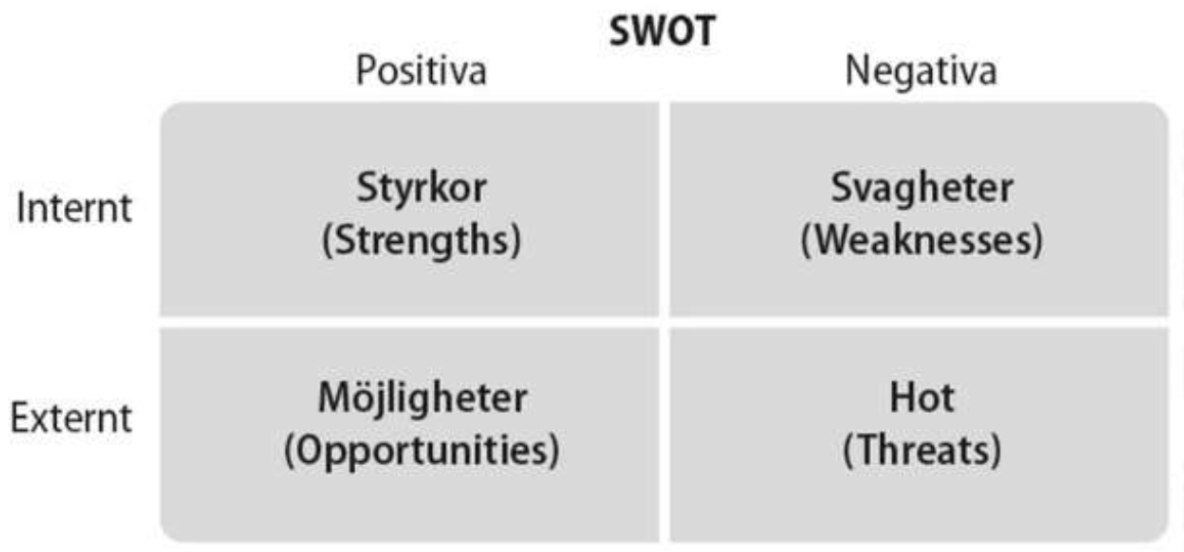
\includegraphics[width=12cm]{\imagesPath/swot.png}
    \caption{SWOT. From \cite{im}}
\end{figure}

\subsubsection{Bostonmatrisen (BCG matrix)}
\begin{figure}[!ht]
    \centering
    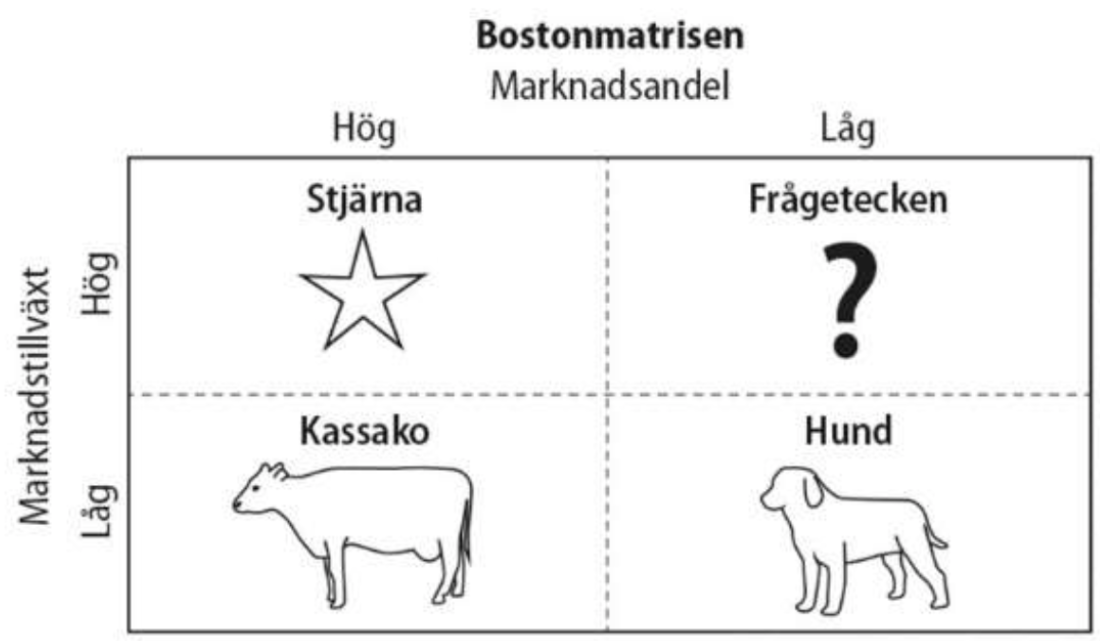
\includegraphics[width=12cm]{\imagesPath/bostonmatrisen.png}
    \caption{Bostonmatrisen. From \cite{im}}
\end{figure}

\newpage
\subsubsection{Produktlivscykeln (Product life cyckle)}
\begin{figure}[!ht]
    \centering
    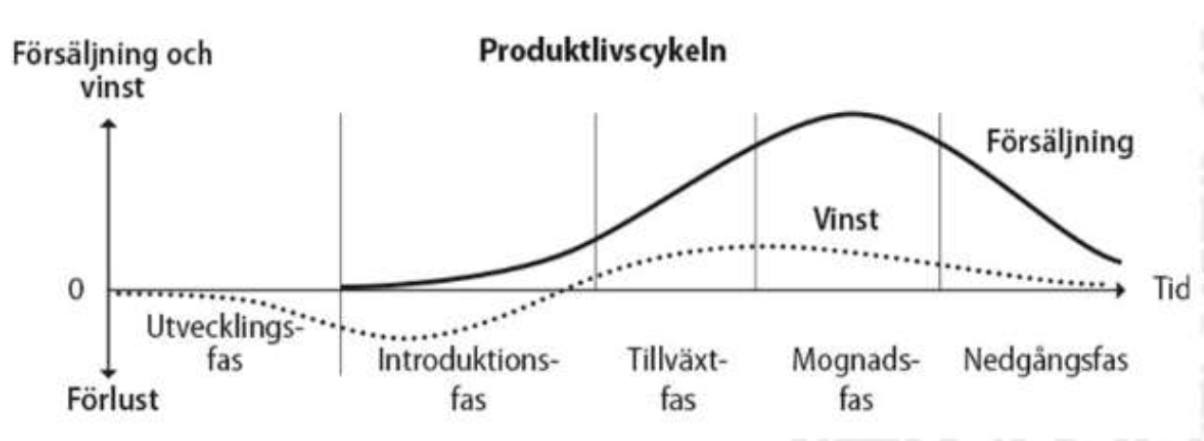
\includegraphics[width=12cm]{\imagesPath/produktlivscykeln.png}
    \caption{Produktlivscykeln. From \cite{im}}
\end{figure}

\subsubsection{Intressentmodellen (Stakeholder analysis)}
\begin{figure}[!ht]
    \centering
    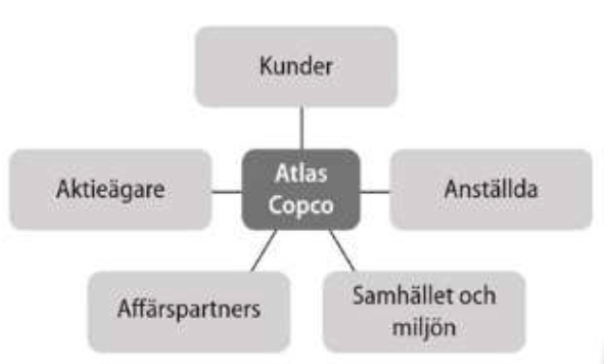
\includegraphics[width=12cm]{\imagesPath/intressentmodellen.png}
    \caption{Intressentmodellen. From \cite{im}}
\end{figure}


\subsection{Ekonomisktyrning (Managment control)}
\begin{itemize}
    \item Styrning av personer
    \item Styrning av kultur
    \item Styrning av resultat
    \item Styrning av agerandet
\end{itemize}

\subsection{Ekonomiskstyrning modeller}
\subsubsection{Det balanserade styrkortet (Balance scorecard)}
\begin{figure}[H]
    \centering
    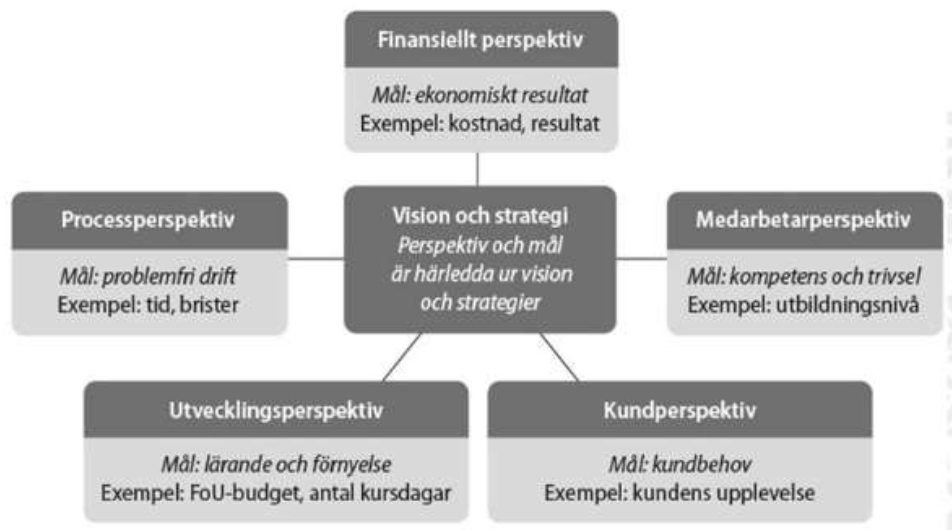
\includegraphics[width=12cm]{\imagesPath/balanserade_styrkort.png}
    \caption{balanserade styrkort. From \cite{im}}
\end{figure}

\begin{multicols}{2}
\subsubsection{Prognoser (Forecasting)}
\begin{itemize}
    \item Försök att se in i framtiden och vad som ska hända då 
    \begin{itemize}
        \item System för planering på olika nivåer
        \begin{itemize}
            \item Aktivetetsplaner
            \item Målstättning
            \item Förväntade värden
        \end{itemize}
        \item Följa trender
        \begin{itemize}
            \item Kritiska frmagångsfaktorer
            \item Nyckelindikatorer
            \item Viktigaste drivarna
        \end{itemize}
    \end{itemize}
\end{itemize}

\subsubsection{Budgetering (Budgeting)}
Budgetering är en \textbf{Handlingsplan} för 
\begin{itemize}
    \item Samordning
    \item Styrning
    \item Kommunikation
    \item Uppföljning och kontroll
\end{itemize}

\textbf{Faser} (uppbyggnad eller nedbrytning)
\begin{enumerate}
    \item Budgetdirektive ges
    \item Budget ställs samman 
    \item Budgetar faställs
    \item Genomförande
    \item Uppföljning
\end{enumerate}

\textbf{Fördelarna} med budgetering
\begin{itemize}
    \item Kan påverka
    \item För delegering
    \item Skapar kostnadsmedvetande
    \item informerar de anställda
\end{itemize}

\textbf{Nackdelar} med budgetering
\begin{itemize}
    \item Tar mycket tid
    \item Slår aldrig in 
    \item Begränsar möjligheter
\end{itemize}

%bostonmatrisen
%productslivscyckeln

%ekonomistyrning
	%typer av styrning: styrning av personer, styrning av kultur, styrning av agerandet, styrning av resultat
	%det balanserade styrkortet

%prognoser
%budgetering


\section{Att agera på marknaden}
\subsection{Typer av marknader}
\begin{itemize}
    \item \textbf{Fullständig (perfekt) konkurrens}: \newline
    Många små företag med samma produkter som därmed konkurrerar med priset
    \begin{itemize}
        \item Den osynliga handen
    \end{itemize}
    \item \textbf{Monopolistisk konkurrens}: \newline
    Väldigt vanlig. Företagen han liknande produkter där vissa kunder föredrar 
    produkter från enna företaget av diverse skäl och därmed konkurerar inte helt
    och hållet på pris.
    \item \textbf{Oligopol}: \newline
    Ett fåtal företag som kontrollerar marknaden. Kan komma överens om pris
    \begin{itemize}
        \item Varning för karteller
    \end{itemize}
    \item \textbf{Monopol}: \newline
    Endast ett företag som kontrollerar marknaden och kan sätta priset själv. 
    \item \textbf{Marknadsekonomi}: \newline
    Det ovanför är typer av marknadsekonomier.
    \item \textbf{Planekonomi}: \newline
    Förekomer oftas i delar av samhälle, som försvaret.
    \item \textbf{Blandekonomi}: \newline
    Kombination av marknadsekonomi och planekonomi.
\end{itemize}

\subsection{Marknadsföring}
\subsubsection{Nätverssynsättet}
\begin{itemize}
    \item \textbf{Bygga upp förtroenden}:
    \item \textbf{Kundlojalitet}:
    \item \textbf{Eftermarknad}: \newline
    Marknad för service och underhåll, reservdelar, tilläggsförsäljning, utbildning 
    med mera till följd av tidigare försäljning av kapitalvaror och industriella produkter
    \item \textbf{Strategiskt partnerskap}: \newline
    Konceptet bygger på att båda parter önskar förstärka en ömsesidig samverkan.
    \item \textbf{Relationsmarknadsföring}: \newline
    innefattar att företag samlar in stora mängder data i olika 
    relationsmarknadsföringsprogram
    \item \textbf{Marknadsföringsplan}: \newline
    Den plan för att planera det följande konsepten
\end{itemize}

\subsubsection{Konkurrensmedel, 4P}
\begin{itemize}
    \item \textbf{Produkt}: Varumärken
    \item \textbf{Pris} 
    \item \textbf{Plats} (Distribution)
    \begin{itemize}
        \item Råvaruindustri > Tillverkningsindustri > Grossist > Detaljist > konsument
    \end{itemize}
    \item \textbf{Promotion} (reklam)
\end{itemize}

\subsection{Strategisk prissättning}
\begin{itemize}
    \item \textbf{Värdebaserad}: (kundbaserad) \newline
    Vad kunden är beräd att betala för den
    \item \textbf{Marknadsbaserad}: (konkurrentbaserad) \newline
    Hur mycket den ska kostnad om man jämför med marknaden
    \item \textbf{Kostnadsbaserad}: \newline
    Hur mycket företaget behöber att den kostar så det går runt.
\end{itemize}
Oftast är det en kombination av de tre.

Producentmarknad (B2B, Business to Business)
\end{multicols}
\raggedcolumns


\subsection{Tjänsteorientering}
\begin{figure}[H]
    \centering
    \includegraphics[width=12cm]{\imagesPath/tjänsteorientering.png}
    \caption{Tjänsteorientering. From \cite{im}}
\end{figure}


\section{Organisera verksamhetern}
\subsection{Typer av hierarkiska organisationer}
\begin{itemize}
    \item \textbf{Linjeorganisation}: (U-form) \newline
    Har den mest tydliga hirarkiska organisationenr med chefer och under chefer sedan arbetare
    \item \textbf{Linje-staborganisation}: \newline
    Är som Linjeorganisation men det har en eller flera så kalande \textit{stab} som 
    är en avdelning som inte ingår i beslutsledet utan mer finns som stöd för övriga enheter, och benämns
    då en linje/stabs-organisation.
\end{itemize}
Operativa enheterna

Det finns också mer produkt fokuserare strukturer som (M-form)
där Divitionerna är olika produkter.

En kombination av linje och produkt fokuserad struktur är MATRIX.
\begin{figure}[H]
    \centering
    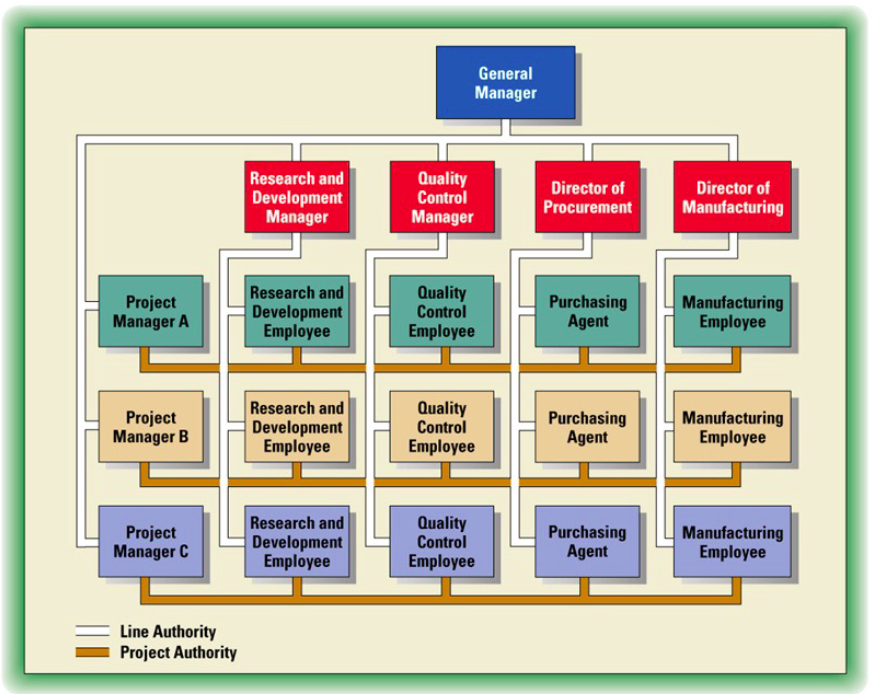
\includegraphics[width=12cm]{\imagesPath/matrix.png}
    \caption{MATRIX. From \cite{im}}
\end{figure}


\begin{multicols}{2}
\subsection{Projektorganisation}
\begin{itemize}
    \item För en uppgift
    \begin{itemize}
        \item Balansera resultat, slutdatum och resurser
    \end{itemize}
    \item Involverar
    \begin{itemize}
        \item Projektledare
        \item Projektägare
        \item Projektgrupp
        \item Projektråd 
        \item Styrgrupp
        \item Delprojekt
    \end{itemize}
    \item Planering
    \begin{itemize}
        \item Indelat iarbetspaket med milsolpar.
        \item Planneras med \textit{PERT} och \textit{CPM} %TODO
    \end{itemize}
\end{itemize}

\subsection{Rerulstatvärdesmetoden}
\begin{align*}
    &\text{Bedömd kostnad vid färdigt} \\
    &= \frac{\text{Faktisk kostnad}}{\text{Resultatvärde}} 
    \cdot \text{Budgeterad total kostnad}
\end{align*}
\begin{align*}
    &\text{Bedömd tid till färdigt} \\
    &= \frac{\text{Planerad kostnad}}{\text{Resultatvärde}} 
    \cdot \text{Budgeterad total tid}
\end{align*}

\subsection{Produktion}
\textbf{Automationsnivå}
\begin{itemize}
    \item Manuell produktion
    \item Semi-automatisk produktion
    \item automatisk produktion
\end{itemize}
\textbf{Volym och variation}
\begin{itemize}
    \item Enstycksprocess
    \item Intermittent (batch) process 
    \item Kontinuerlig process
\end{itemize}

\subsubsection{Layout i lokalen}
\begin{itemize}
    \item Fast position 
    \item Funktionell layout: Placering utifrån aktivitet i produktionen
    \item Födesgrupper: celler 
    \item Linjebaserad layout: produktorienterad placering
\end{itemize}

\subsection{Lager Optimering}
\begin{align*}
    &\text{Optimal inköpskvantitet} \\
    &= \sqrt{\frac{ 2\cdot\text{Efertågan per år}\cdot\text{ordersärkostnad per order} }{ \text{Lagerhållningskostnad per styck} }}
\end{align*}

\begin{figure}[H]
    \centering
    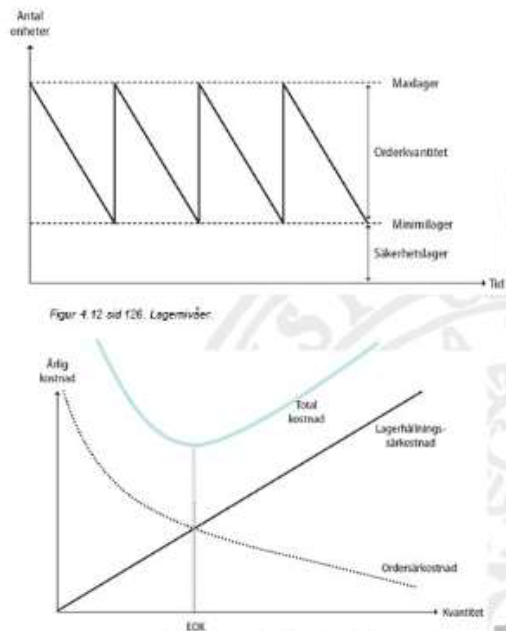
\includegraphics[width=8cm]{\imagesPath/lager_optimering.png}
    \caption{lager optimering grapher. From \cite{im}}
\end{figure}

\begin{exampleblock}{Exempel WrapUp AB}
   TODO 
\end{exampleblock}

\subsection{Vad gör en ledare?}
\begin{itemize}
    \item \textbf{Mintzberg}
    \begin{itemize}
        \item Interpersonella rollen: \newline
        Representant, vägledare och nätverkare
        \item Informationsrollen: \newline
        Övervakare, informationsspridare och talesperson
        \item Beslutsrollen: \newline
        Entreprenör, problemhanterare, resursfördelare och förhandlare
    \end{itemize}
    \item \textbf{Hamel}
    \begin{itemize}
        \item Formulera och planera målförverkligande
        \item Motivera och samordna insatser
        \item Koordinera och styra aktiviteter
        \item Utveckla och tillsätta talanger
        \item Ackumulera och applicera kunskap
        \item Anskaffa och fördela resurser
        \item Skapa och vårda relationer
        \item Balansera och tillmötesgå krav från investerare
    \end{itemize}
\end{itemize}

\subsubsection{Bolagets ledning}
\begin{itemize}
    \item Bolagsstämma 
    \begin{itemize}
        \item Aktieägarna
        \item Högsta beslutande organ
    \end{itemize}
    \item Högsta ledningen
    \begin{itemize}
        \item Styrelsen: \newline
        Ansvarar för organisation och förvaltning
        \item Företagsledningen: \newline
        VD: löpande förvaltning
    \end{itemize}
    \item Mellanchefer
    \item Operativa chefer
    \begin{itemize}
        \item Första linjens chefer 
        \item Arbetsledare
    \end{itemize}
\end{itemize}

\subsubsection{Ansvar}
\begin{itemize}
    \item Räntabillitetsansvar (Investment center): (intäkt - kostnad)/ Kapital \newline
    Exempelvis: CEO
    \item Resultatansvar (Profit center): Intäkt - Kostnad \newline
    Exempelvis: 
    \item Intäktsansvar (Revenue center): Intäkter och kostnad \newline
    Exempelvis: Key accountant manager
    \item Kostnadsansvar (Cost center): Kostnad  \newline
    Exempelvis: Chef ekonomi ansvarig
    \item Timansvar (Hour center): Timmar \newline
    Exempelvis: Lathe manager
\end{itemize}
\end{multicols}
\raggedcolumns


%lager optimering
%EOK ekonomisk order kostnaden, lagerhålnings kostnaden
%ex
%
%sedan ledarskap
%fins mer tolkining med flöde men också som pukter
%
%Bolags styrning. Hur företaget styrs
%
%Olika andvar i företaget
%
%Läranden, det olika former och hur de kan utvercka medarbetare

\section{Kalkyler för produkter och order}
\subsection{Begrepp i flödet}
\begin{figure}[H]
    \centering
    \includegraphics[width=12cm]{\imagesPath/begrepp_i_flödet.png}
    \caption{Begrepp i flödet. From \cite{im}}
\end{figure}

Inbetalning är när vi får pengarna på banken 
Inkomst är hur mycket våra kunder att betala oss 
Intäkt?

\subsubsection{Periodisering}
För att mäta produkts resultat så räknar vi resursenrna som krävdes för produkten 
(kostnad) och gemför dessa med hur produkten presterade (intäkt).
Periodisera betyder att det är gjämförbara. 

\subsection{Kalkylbegrepp}
\begin{figure}[H]
    \centering
    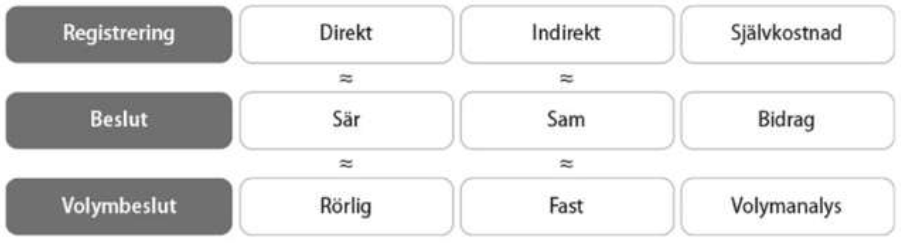
\includegraphics[width=12cm]{\imagesPath/kalkylbegrepp.png}
    \caption{Kalkylbegrepp. From \cite{im}}
\end{figure}
\begin{itemize}
    \item Direkt kostnad: Kostnad spesific för produkten
    \item Indirekt kostnad: Kostnad som är delvis för den produkten (lathe)
    \item Särintäkter: Sär är relevant kostnad 
    \item Samintäkter: Sam är irelevant kostnad.  
    \item Rörlig kostnad: Förändrar sig med antal enhetet
    \item Fast kostnad: Är alltid samma
\end{itemize}


\subsection{Kalkylmodeller}
Det finns kalkyler som görs före och efter beslut.
\begin{figure}[H]
    \centering
    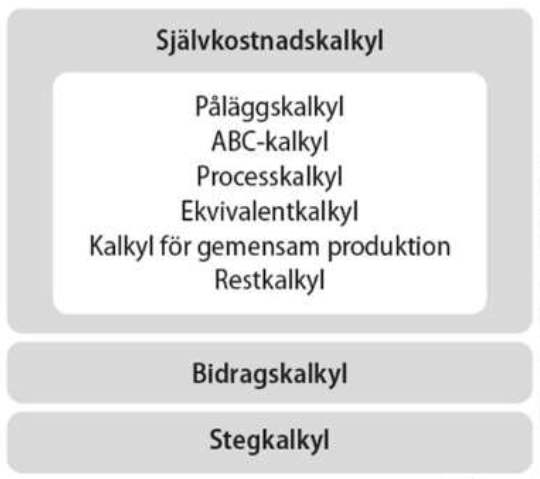
\includegraphics[width=12cm]{\imagesPath/kalkylmodeller.png}
    \caption{Kalkylmodeller. From \cite{im}}
\end{figure}


\newpage
\subsection{Påläggskalkyl}
\begin{figure}[H]
    \centering
    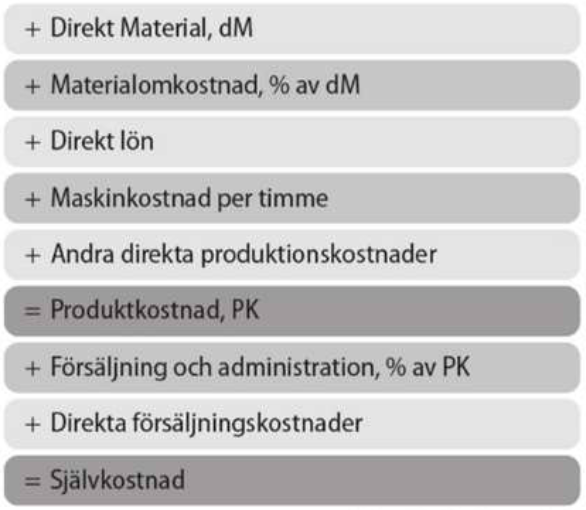
\includegraphics[width=12cm]{\imagesPath/påläggskalkyl.png}
    \caption{Påläggskalkyl. From \cite{im}}
\end{figure}

\begin{exampleblock}{Exempel Savox AB}
   Savox AB utför diverse lackeringsuppdrag för andra företag. För år 2018 har de 
   budgeterat en direkt materialkostnad på 1 400 000 kronor, materialomkostnader på 
   280 000 kronor, direkta löner i produktionen på 400 000 kronor, indirekta produktionskostnader 
   på 880 000 kronor för den planerade maskintiden 8 800 timmar, andra direkta 
   produktionskostnader på 40 000 kronor, direkta försäljningskostnader på 100 000 kronor, 
   och försäljning och administration på 1 200 000 kronor. Nu har företaget fått en order för 
   lackering av en plastdetalj. För detta behövs färg för 5 000 kronor, 5 direkta 
   arbetstimmar i produktionen vilka vardera kostar 1 200 kronor, 10 maskintimmar och en 
   direkt försäljningskostnad på 1 000 kronor. 

   a. Till vilket belopp uppgår företagets självkostnad enligt budget?
   b. Vilka pålägg och timkostnader bör företaget använda under året? 
   c. Vad är kostnaden för den order de nu fått? 

   ... %TODO
\end{exampleblock}

%F;r Inderekta kostnader så har man prosuent.
%
%Först räkna pålägskalyl
%sedan andvända dessa för kalkylering av olika order och liknade under perioden.
%
%
%Exempel

\newpage
\subsection{Aktivitetsbaserad kalkyl, ABC}
\begin{figure}[H]
    \centering
    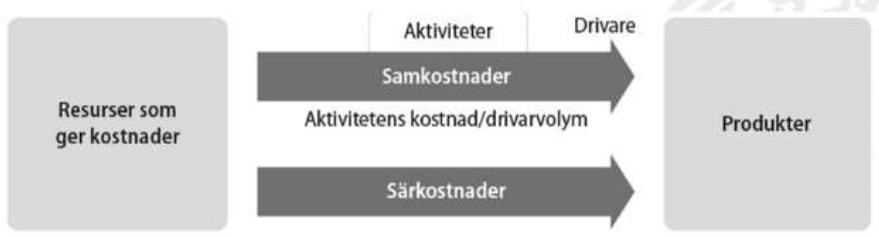
\includegraphics[width=12cm]{\imagesPath/abc.png}
    \caption{ABC. From \cite{im}}
\end{figure}

\begin{exampleblock}{Exempel Savox AB-C}
    Savox AB har bestämt sig för att använda en del ABC i sitt kalkylsystem. Jämför 
    denna övning med den föregående, där de använde en påläggskalkyl. För år 2018 har de 
    budgeterat en direkt materialkostnad på 1 400 000 kronor, materialhantering för 280 000 
    kronor med liter färg som drivare, produktion som kostar 400 000 kronor, maskinbearbetning 
    som kostar 880 000 kronor för den planerade maskintiden 8 800 timmar, andra direkta 
    produktionskostnader på 40 000 kronor, direkta försäljningskostnader på 100 000 kronor, 
    försäljningsaktiviteter för 400 000 kronor med antal order som drivare, vilket beräknas till 400 för 
    året, samt försäljning och administration för 800 000 kronor för vilket de inte finner en lämplig 
    drivare och vilket de inte anser orsakas av order som sådana. Nu har företaget fått en order för 
    lackering av en plastdetalj. För detta behövs 140 liter färg för 5 000 kronor, 5 direkta arbetstimmar i 
    produktionen vilka vardera kostar 1 200 kronor, 10 maskintimmar och en direkt försäljningskostnad 
    på 1 000 kronor.

    a. Till vilket belopp uppgår företagets självkostnad enligt budget?
    b. Vilka kostnader per drivare bör företaget använda under året? 
    c. Vad är kostnaden för den order de nu fått? 

   ... %TODO
\end{exampleblock}
%ger b'ttre bed;mning 'n p[l'gskalkyl men inte perfekt
%
%aktivitet och drivare
%Exempel


\newpage
\subsection{Bidragskalkyl (Contribution Margin Costing)}
\begin{figure}[H]
    \centering
    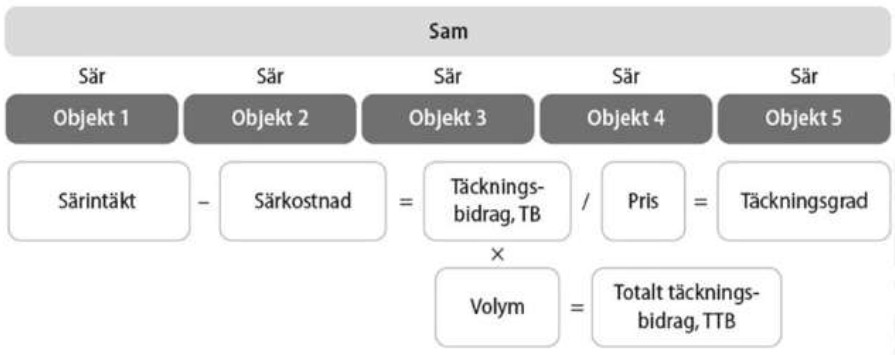
\includegraphics[width=12cm]{\imagesPath/bidragskalkyl.png}
    \caption{Bidragskalkyl. From \cite{im}}
\end{figure}
Särintäkt pris som betalt för produkten och särkostnaderna är vad det kostar att producera.
räkningsgrad beteknas som bruttomarginal.

\subsubsection{Beslut}
Med bidragskalkylen så kan man andvända den till att fatta vissa beslut som:
\begin{itemize}
    \item Ska ordern accepteras? \newline
    Tar endast hänsyn till beslutrelevanta, orderspecifika effekter på sikt
    \item Produktval vid en begränsnig (en trång sektion) \newline
    Den produkt som ger högst TTB, d.v.s högst TB per trång sektion, bör väljas
    \item Produktval vid flera begränsningar (flera tånga sektioner) \newline
    Den kombination av produkter som ger högst TTB, enligt t.ex. linjär programmering, bör väljas
    \item Allmäna beslut om förändringar \newline
    Tar endast hänsyn till beslutrelevanta, förändringsspecifika effekter på kort sikt
\end{itemize}


\begin{exampleblock}{Exempel ChoicesAB}
    todo
    
    Endast särkostnaden är relevant för beslutet. Tex så tar man inte in ens egna hyran i 
    beräkningen för pris på en biobiljet är värt det eller inte.
\end{exampleblock}

\subsection{Stegkalkyl}
\begin{figure}[H]
    \centering
    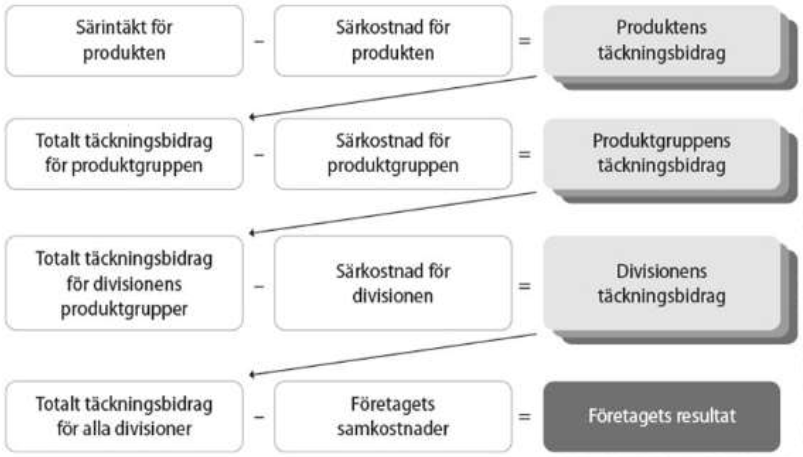
\includegraphics[width=12cm]{\imagesPath/stegkalkyl.png}
    \caption{Stegkalkyl. From \cite{im}}
\end{figure}


\subsection{Andra självkostnadskalkyler}
Exempel

\section{Investeringsbeslut}

Grundprincip: Insättning på bank
\begin{itemize}
    \item Ränta på ränta, slutvärde: Kapital $\times (1+r)^n$
    \item Nuvärde: Kapital $\times \frac{1}{(1+r)^n}$
    \item Nuvärdesumma: Kapital $\times \frac{1-(1+r)^{-n}}{r}$
    \item Annuitet: Kapital $\times \frac{r}{1-(1+r)^{-n}}$
\end{itemize}

\begin{figure}[H]
    \centering
    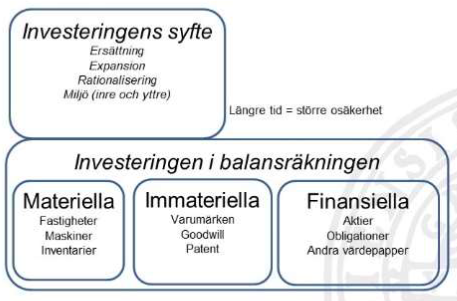
\includegraphics[width=12cm]{\imagesPath/typer_av_investeringar.png}
    \caption{Typer av investeringar. From \cite{im}}
\end{figure}

\begin{figure}[H]
    \centering
    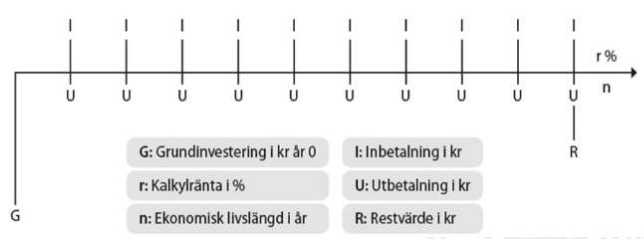
\includegraphics[width=12cm]{\imagesPath/kalkylbegrepp_investering.png}
    \caption{Kalkylbegrepp. From \cite{im}}
\end{figure}

\begin{figure}[H]
    \centering
    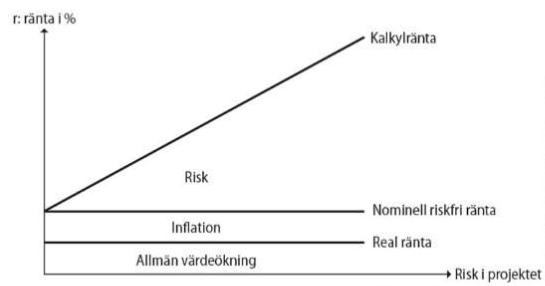
\includegraphics[width=12cm]{\imagesPath/kalkylrantan.png}
    \caption{Kalkylräntan. From \cite{im}}
\end{figure}

Metoder för investering 
\begin{itemize}
    \item Nuvärdemetoden
    \begin{itemize}
        \item Positivt = lönsamt, ju högre desto bättre
        \item Kan endast jämföra investeringar med samma ekonomiska livslängd
    \end{itemize}
    \item Annuitetsmetoden
    \begin{itemize}
        \item Positivt = lönsamt, ju högre desto bättre
    \end{itemize}
    \item Internräntemetoden
    \begin{itemize}
        \item Ju högre internränta desto bättre 
        \item Testa, eller dela grundinvesteringen med det årliga betalningsöverskottet
        \item Kan bara använda om det också finns inbetalningar
    \end{itemize}
    \item Återbetalningtid (pay-back)
    \begin{itemize}
        \item $\sum$ inbetalningsöverskott $=$ Grundinvesteringen, eller Grundinvestering/årligt inbetalningsöverskott
        \item Ju kortare tid desto bättre
        \item Problem; kortsiktigt, ingen ränta (i grundversionen)
    \end{itemize}
    \item Investeringens räntabilitet
    \begin{itemize}
        \item Genomsnittligt årligt inbetalningsöverskott divideras med genomsnittlig investering 
        \item Ju högre procent räntabilitet desto bättre 
        \item Problem: Tar inte hänsyn till ränta
    \end{itemize}
\end{itemize}


%ekonomisk livslängd: när det kommer betalas av.
%arr 

shabloner, prusent (enkla)
aktivitetbaserad kalkyl 

-----

Balanse tekning
inventarie, sånt som inte ändrar sig

nuvärde
annueitet
återbetalningid

Teknisk livslängd är så länge som en anläggning (eller del av anläggning) går att tekniskt/funktionellt att använda. Ekonomisk livslängd är den tid som det är ekonomiskt rationellt att använda anläggningen


kalkylränta är riks, real ränta och inflation
real ränta hur det faktiskt förändras

återbetalningen metoden är inte riktigt rätt

räntan är inte bankräntan

\section{Uppföljning av verksamheten}

\textbf{Bokföring med T-konton}
\begin{figure}[H]
    \centering
    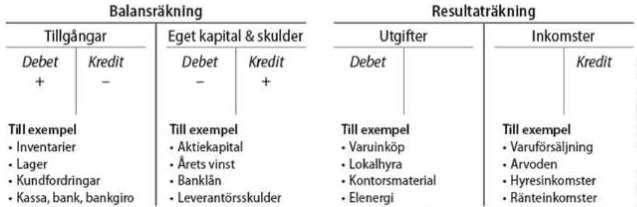
\includegraphics[width=12cm]{\imagesPath/bokforing_med_t-konton.png}
    \caption{Bokforing med t-konton. From \cite{im}}
\end{figure}
notera att kredit och debit för balansräkningen respektive resultaträkningen ska vara samma.
Debet betyder enbart vändstra sidan av räkningarna och Kredit är högra.
Var man lägger tillgångar samt eget kapital \& skulder respektive Utgifter och incomseter är 
upptill företaget. Men skenerält så är det rällativt licka sätt man lägger up det.

\begin{itemize}
    \item SCOA2
    \item Kiosk är en ..
    \item FAST rapport
    \item årsredovisning
    \item årsmöte
\end{itemize}

\textbf{Årsredovisningens innehåll}
\begin{figure}[H]
    \centering
    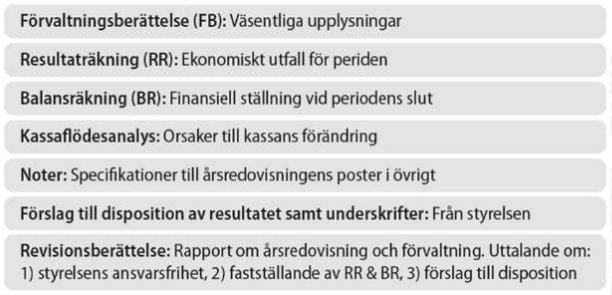
\includegraphics[width=12cm]{\imagesPath/arsredovisningens_innehall.png}
    \caption{Årsredovisningens innehåll. From \cite{im}}
\end{figure}

\textbf{Resultaträkning och balansräkning}
\begin{figure}[H]
    \centering
    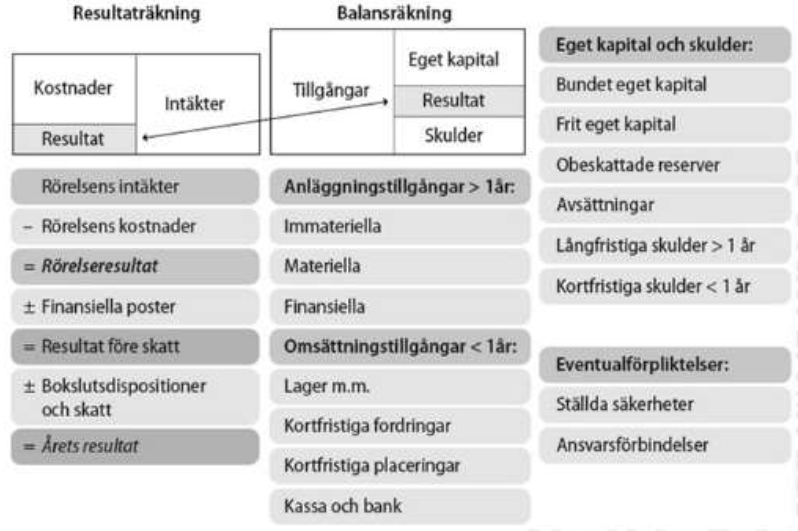
\includegraphics[width=12cm]{\imagesPath/resultatrakning_och_balansrakning.png}
    \caption{Resultaträkning och balansräkning. From \cite{im}}
\end{figure}

\subsection{Redovisningens regler}
\begin{itemize}
    \item Lagar och regelverk
    \begin{itemize}
        \item Bokföringslagen, Aktiebolagslagen, Årsredovisningslagen, Inkomstskattelagen.
        Mervärdeskattelagen, Skattebetalningslagen m.m.
        \item Svensk kod för bolagsstyrning, Sarbanes-Oxley Act SOX 
    \end{itemize}
    \item Redovisningens principer
    \begin{itemize}
        \item Rättvisande bild, "true and fair view"
        \item Periodisering, fortlevand, jämförbarhets, försiktighet, realisering, osv
    \end{itemize}
    \item Normgivare: God redovisningssed
    \begin{itemize}
        \item Bokföringsnämnden, Rådet för finansiell rapportering, FAR SRS 
        \item IASB (Eng) International Accounting Standards Board med IFRS (International Financial Reporting Standards)
        \item FASB (USA) Financial Accounting Standards Board
    \end{itemize}
\end{itemize}

Revisorn jobbar för aktieägarna. Det måste se till att det siffror som aktie ägarna får(redovisas) 
är rätt.

Namn och begrepp måste vara med och för årsredovisning

Det går att ändra räkenskapsår, men man måste anmäla att göra en sån ändring


\subsection{Måt}
\begin{itemize}
    \item Omsättingstillgångar: Lägsta värdets princip (försiktighetsprincip). Är tillgångar som förväntas säljas om ett år.
    \item Anläggningstillgångar: Långtids investeringar, mer än 1 år
    \item Värdering och bokslutsdisponitioner: %TODO
\end{itemize}

EBITDA är ett annat finnansielt mått.

\begin{itemize} %TODO update with what they mean
    \item Soliditet: överlevnadsförmåga \newline
    $\frac{\text{Eget kapital}}{\text{Totalt kapital}}$
    \item Balanslikviditet: \newline 
    $\frac{\text{Omsättningstillgångar}}{\text{Kortfristiga skulder}}$
    \item Kassalikviditet: \newline
    $\frac{\text{Omsättningstillgångar minus lager}}{\text{Kortfristiga skulder}}$
\end{itemize}

Lösamhet (räntabilitet)
\begin{itemize}
    \item Räntabilitet på egen kapital, $R_E$: ägarnas avkastning \newline
    $\frac{\text{Årets resultat}}{\text{Genomsnittligt eget kapital}}$
    \item Räntabilitet på totalt kapitel, $R_t$: total avkastning \newline
    $\frac{\text{Resultat före skatt plus finansiella kostnader}}{\text{Genomsnittligt totalt kapital}}$
\end{itemize}

DuPoint-formeln
\begin{figure}[H]
    \centering
    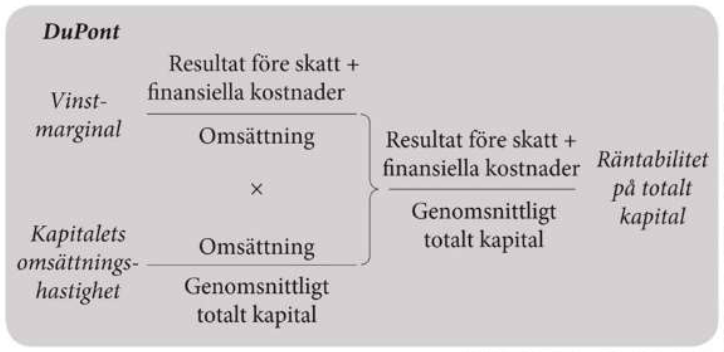
\includegraphics[width=12cm]{\imagesPath/DuPoint-formeln.png}
    \caption{DuPoint-formeln. From \cite{im}}
\end{figure}

exampels %TODO

%Balansräkning räckas när vi inte hanterar inbetalningar och utbetalningar utan att
%vi har tillgångar eller att vi lovar att betala i form av skuld

Vi har stabilt näringsiv i sverige. Vi har regler som skattar mycket när det går bra 
och lite när det går dårligt 

Värde på tillgångar är upp till företaget att välja innom vissa sätta rammar som är samma för alla

Om man inte anmäler om konkurs när soliditet är för lågt så kommer man vara skildig till 
att betala ur egen plånbock. 

%kumodurater monga verksamheter DuPoint

Man har förökt redovisa hållbarhet, dock så har det inte kommigt så långt med det.


\section{Analysera förändring}
Rörliga kostnader
\begin{itemize}
    \item Rörlig kostnad: rack linje (Kronor totalt x volym)
    \item Avtagande rörliga kostnader: avtagande ökande kurva (kronor totalt x volym)
    \item Ökande rörliga kostnader: exponentiel kurva (kronor totalt x volym)
\end{itemize}

Fasta kostnader 
\begin{itemize}
    \item Fast kostnad: horizontelt sträck (kronor, totalt x Volym)
    \item Halvfast kostnad: ökar stegvis beronde på volym
    \item Halvfast kostnad: blir biligare per styck ju störe volym men ökar vid en viss mängd, blir som en såg kurva
\end{itemize}

Volymanalys 
\begin{figure}[H]
    \centering
    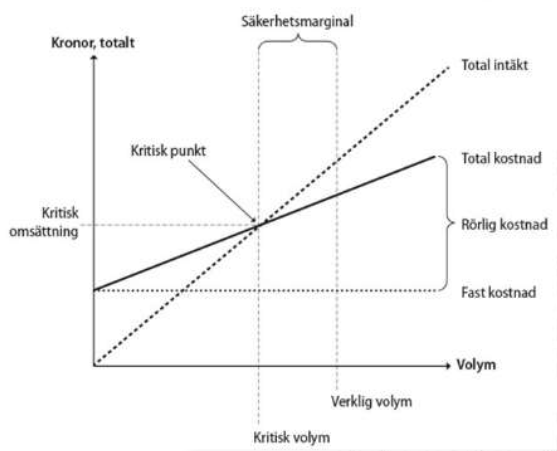
\includegraphics[width=12cm]{\imagesPath/volymanalys.png}
    \caption{Volymanalys. From \cite{im}}
\end{figure}

\begin{exampleblock}{Exempel: Fasta Rör AB}
    Företaget Fasta Rör AB säljer en produkt för 20 kronor per styck. Man hade i januari en 
    total kostnad på 1 630 000 kronor, och i februari en total kostnad på 1 930 000 kronor. Inga 
    andra skillnader noterades mellan perioderna än att volymen uppgick till 82 000 enheter i januari 
    och till 102 000 enheter i februari.
\end{exampleblock}

\begin{itemize}
    \item Direct costs: Costs that can directly ried to the production of specific goods or services.
    Ex: Direct labour and material.
    \item Inderect costs: Costs that are neccessary, but dificult to trace to the cot object. 
    Ex: Overhead (rents, utulities, administation)
    \item Relevant costs: Costs that are affected by managerial choice in a cerain business situation.
    Ex: Variable or marginal costs, increamental costs, specific costs, avoidable ficed costs, oppertunity costs.
    \item Irrelevant costs: costs that won't be affected by a managerial decision.
    Ex: Sunk costs and costs which are same for different alternatives.
    \item Fixed costs: Costs that change in total when the volume changes.
    Ex: Rents, insurance, employee salaries, etc.
    \item Variable costs: Costs that don't change in total when the volume is changing.
    Ex: Sunk costs and costs which are same for different alternatives.
\end{itemize}

\begin{center}
    Total Cost = Fixed Costs + Variable Costs
\end{center}

Fundamental equaion 
\begin{center}
    Operating Profit = Revenues - Total VC - Total FC
\end{center}

\section{Verksamhetens finansiering}
Kapitalbehov 
\begin{figure}[H]
    \centering
    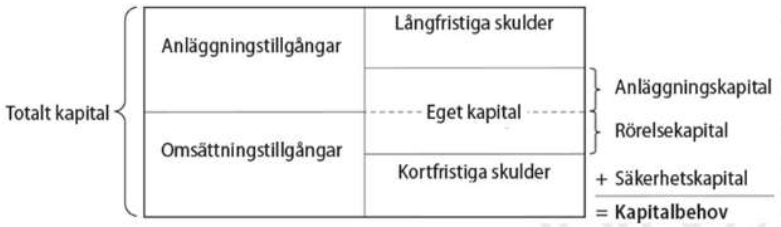
\includegraphics[width=12cm]{\imagesPath/total_kapital.png}
    \caption{Kapitalbehov. From \cite{im}}
\end{figure}

Olika typer av Risker 
\begin{itemize}
    \item Verksamhetsrisker
    \begin{itemize}
        \item Risker på grund av verksamheten
        \item till exempel marknadsrisk, tillverkningsrisk, leverantörsrisker, och så vidare
    \end{itemize}
    \item Finansiella risker 
    \begin{itemize}
        \item Risker till följd av hur investeringarna finansieras
        \item till exempel risken för förändringar i valutakurserna, risken för förändringar i det funanaiella nettot, och risken för nya skatteregler.
    \end{itemize}
\end{itemize}

\textit{Kapitalrationalisering} går ut på att förbättra ett företags räntabilitet genom en förbättrad kapitalomsättning
\subsection{Anläggningskapital (Fixed capital)}
describes a company's investment in long-term assets - relatively permanent 
- e.g., for property, plant and equipment on the balance sheet

\subsection{Rörelsekapital (Working capital)}
is the amount of available capital that a company can readily use for 
day-to-day operations (measures a company's liquidity, operational effeciency,
short-term finnancial health) - e.g., for inventory, accounts receivables, etc.
\textit{Rörelsekapital}
\begin{itemize}
    \item Procentmetoden
    \begin{itemize}
        \item Procentuell ändring i posterna p g a t.ex. omsättningsökning
    \end{itemize}
    \item Genomsnittsmetoden
    \begin{itemize}
        \item Kundfordringar = (kredittid i dagar/360 dagar) $\times$ försäljning
        \item Leverantörsskulder = (kredittid i dagar/360 dagar) $\times$ inköp
        \item Förråd = (minimilager + maximilager)/2 (eventuellt sen $\times$ kronor)
        \item Produkter i arbete i kronor = Antal produkter $\times$ halva produktkostnaden
        \item Färdiglager i kronor = Antalet produkter $\times$ produktkostnaden
    \end{itemize}
    \item Resursmetoden och balansräkningsmetoden 
\end{itemize}

\subsection{Safety capital}
Amount of capital to cover for variations in sales and the like.

\subsection{Other terminology}
\textit{Resursmetoden}
\begin{figure}[H]
    \centering
    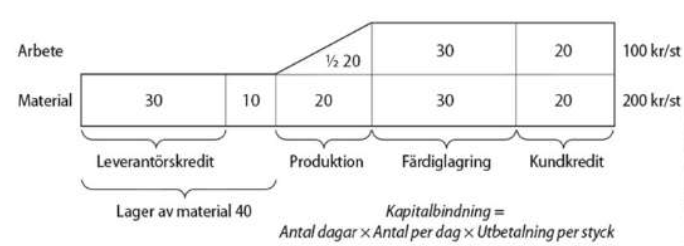
\includegraphics[width=12cm]{\imagesPath/resursmetoden.png}
    \caption{Resursmetoden. From \cite{im}}
\end{figure}

\textit{Kreditmarknaden} \newline
Främmande kapital kreditmarknad:
\begin{itemize}
    \item Obligationslån
    \item Inteckningslån 
    \item Reverslån 
    \item Kontokredit 
    \item Factoring
    \item Leasing 
    \item Konvertibla skuldebrev
\end{itemize}

\textit{Aktiemarknaden} \newline
Eget kapital Aktiemarknad
\begin{itemize}
    \item Sparade vinster 
    \item Nyemission: fler aktie, för att göra det biligare att handla med aktien
\end{itemize}

\subsection{Analyser}
\textit{kassaflödes analys}
\begin{figure}[H]
    \centering
    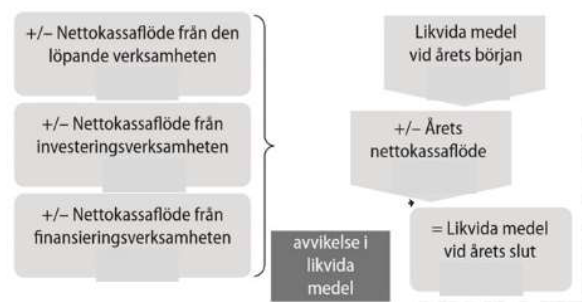
\includegraphics[width=12cm]{\imagesPath/kassaflodesanalys.png}
    \caption{Kassaflödesanalysens komponenter. From \cite{im}}
\end{figure}

\textit{Finansiell analys}
\begin{figure}[H]
    \centering
    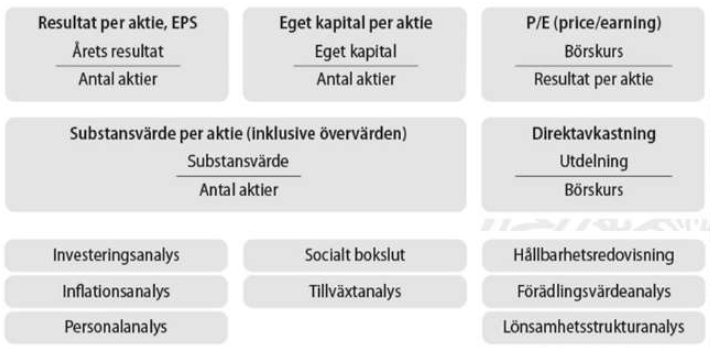
\includegraphics[width=12cm]{\imagesPath/finnansiell_analys.png}
    \caption{Kassaflodesanalys. From \cite{im}}
\end{figure}

Bank will get the money before the shareholder in case of bankrupsy
